\documentclass[conference,letter]{IEEEtran}
\usepackage{url}
\usepackage{graphicx}
\usepackage{subfigure}

\newcommand{\todo}[1]{\textbf{TODO}\footnote{\textbf{TODO:} #1}}

\begin{document}

\title{The GHTorent Dataset and Tool Suite}

\author{\IEEEauthorblockN{Georgios Gousios} 
\IEEEauthorblockA{
Software Engineering Research Group\\
Delft University of Technology\\
Delft, The Netherlands\\
g.gousios@tudelft.nl}
}

\maketitle

\begin{abstract} 
  
  During the last few years, GitHub has emerged as a popular project hosting,
  mirroring and collaboration platform. GitHub provides an extensive {\sc rest
  api}, which enables researchers to retrieve high-quality, interconnected data.
  The {\sc ght}orent project has been collecting data for all public projects
  available on Github for more than a year. In this paper, we present the dataset
  details and construction process and outline the challenges and research
  opportunities emerging from it.

\end{abstract}

\begin{IEEEkeywords}
dataset, repository, GitHub
\end{IEEEkeywords}

\section{Introduction} During the recent years, Github has become the repository
hosting site of choice for many Open Source Software ({\sc oss}) projects.
Interestingly, Github provides a {\sc rest api} to its full data set, making it
an attractive research target. The {\sc ght}orent project uses the Github {\sc api}
to collect raw data and extract, archive and share queriable metadata. The
created datasets have already been exploited in other work (analysis of the pull
development model~\cite{GPD13}, analysis of drive-by commits and analysis of
test incentives on social sites),
while collaborations with external research groups are under way. 

An outline of the project and bits of the implementation were presented
in~\cite{GS12}. Since this work, we extended the collection process to an
additional 15 {\sc api} end points, stabilized the data and metadata schema and
developed a service to collaboratively collect and share data. More than 900{\sc
gb} of raw data and 10{\sc gb} of metadata have been collected and are available
for download. In this paper, we present the finalized schema, go through the
challenges and limitations of working with the dataset and outline research
opportunities that emerge from it.

\begin{figure*}
  \footnotesize
  \begin{center}
    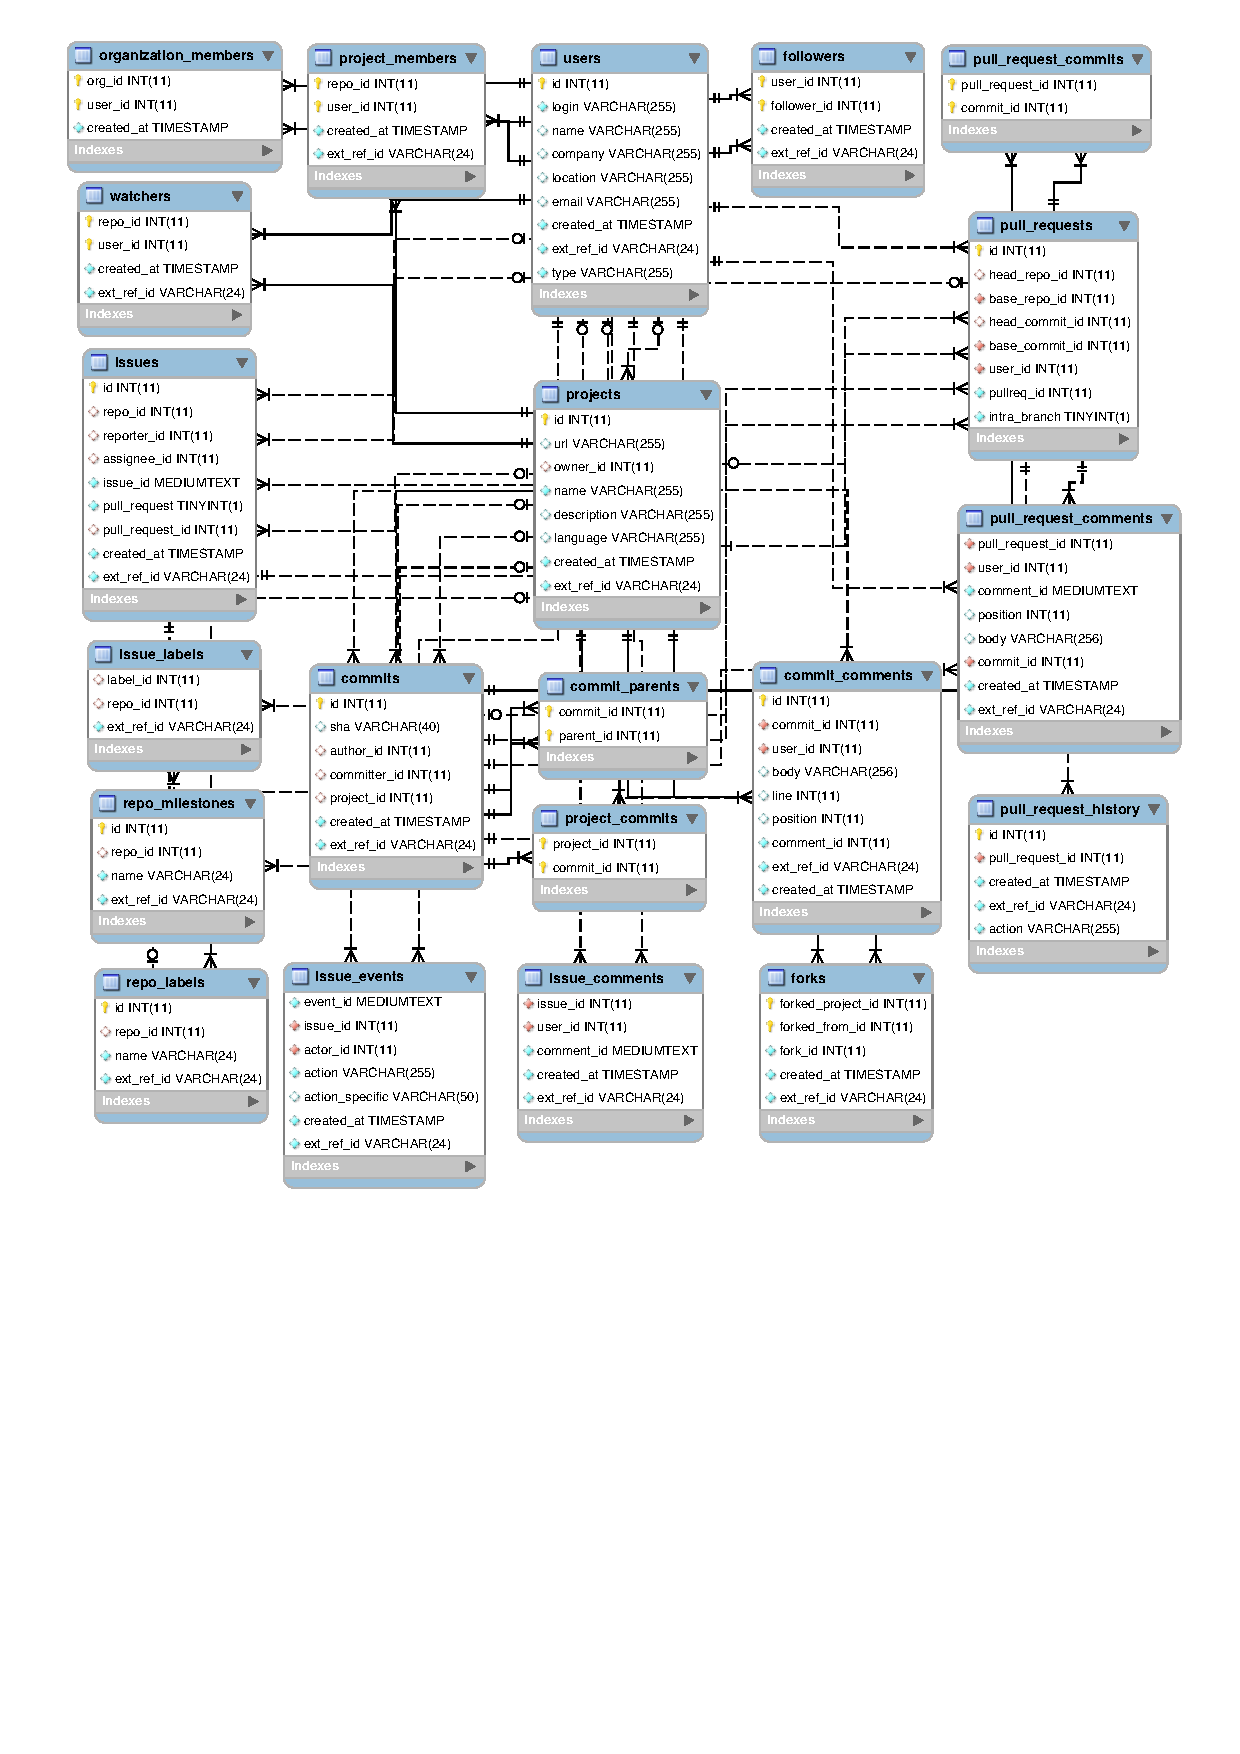
\includegraphics[scale=0.83]{ghtorrent-schema.pdf}
  \end{center}
  \centering
  \begin{tabular}{lp{25em}p{8em}l}
      \hline
      \bf{Entity} & \bf{Description} & \bf{Raw data entity} & \bf{Num Items} \\
      \hline
      --- & Events on repositories. & \texttt{events} & 43,090,195\\

      \sf{projects} & Project repositories. & \tt{repos} & 1,326,900\\
      
      \sf{users} & Github users. & \tt{users} & 793,855\\

      \sf{project\_members} & Users with commit access to the referenced
      \sf {project}. & \tt{repo\_collabs} & 983,629\\
      
      \sf{organization\_members} & List of members in an organization. & \tt{org\_members} & 34,924\\

      \sf{commits} & A list of all commits on Github. The {\tt project\_id} field
      refers to the first {\sf project} this commit has been added to. &
      \tt{commits} & 29,978,291\\
      
      \sf{project\_commits} & List of all \sf{commits} to a \sf{project}.& --- &
      ---\\

      \sf{commit\_parents} & Commits that are parents to a {\sf commit}.& --- & ---\\
      
      \sf{commit\_comments} & Code review comments for a {\sf commit}.& \tt{commit\_comments} & 126,697 \\
      
      \sf{watchers} & {\sf user}s that have starred (was watched) a {\sf project} & \tt{watchers} & 7,744,619\\

      \sf{followers} & {\sf user}s that are following another \sf{user}. & \tt{followers} & 1,797,343\\

      \sf{issues} & Issues that have been recorded for a \sf{project}.&
      \tt{issues} & 2,326,069 \\
      
      \sf{issue\_events} & Chronologically ordered list of events on an
      \sf{issue}. & \tt{issue\_events} & 4,085,294\\
      
      \sf{issue\_comments} & Discussion comments on an \sf{issue} &
      \tt{issue\_comments} & 2,886,006\\
      
      \sf{pull\_requests} & List of pull requests for {\sf base\_repo}. Requests
      originate at head {\tt head\_repo}/{\tt commit} and are created by
      {\tt user\_id} & \tt{pull\_requests} & 1,144,251 \\ 
 
      \sf{pull\_request\_comments} & Discussion comments on a \sf{pull\_request}
      & \texttt{pullreq\_comnts} & 2,228,894\\

      \sf{pull\_request\_history} & Chronologically ordered list of events
      on a \sf{pull\_request} & --- & ---\\

      \hline
    
  \end{tabular}
  \caption{Schema entities, their description, the corresponding raw data
  entities and the number of raw data items (Feb 15, 2013).}
  \label{fig:entities}
\end{figure*}

\section{Data Collection}

The primary challenge for the data collection process is the Github imposed
5,000 requests per hour limit for authenticated requests, while the event
generation rate is already higher;\footnote{On an average day, Github produces
200,000 events, or about 8,300 events per hour} given that a single event can
lead to several (even thousands) of dependent requests, it is not
practical to assume that a single Github account will suffice to mirror the whole
dataset. For this reason, {\sc ght}orent was designed from the ground up to use caching excessively (to avoid duplicate requests) and also to be distributed (to 
enable multiple users to retrieve data in parallel). We briefly
describe how {\sc ght}orent employs those two mechanisms in the following paragraphs.

The Github {\sc api} supports two types of queries:

\begin{itemize}

  \item Resource queries retrieve a specific instance of a resource. Per 
    {\sc rest} architecture mandates, the {\sc url} identifying a static
    resource remains constant after the resource has been initialized. 

  \item Range queries retrieve a list of resources, usually related to a given
    resource. For example, the query \texttt{/\{user\}/followers} retrieves the
    followers for a user, while the query \texttt{/\{user\}/\{repo\}/commits}
    retrieves the commits for a repository. Paging is used to limit the amount
    of data per response. Range queries do not necessarily return the full
    entity instance for each item, but they usually include a {\sc url} where
    the item may be retrieved. As a result, a range query might result to
    several resource queries.

\end{itemize}

Resource query results can be cached very efficiently, as by definition they
never change. Range queries are trickier to cache, as their result might change
as the project evolves (new commits, new followers, etc); fortunately, by
default Github serves newer results first, so it is enough to go through the
first few pages of results only in order to retrieve the updated data. To cache
the results per entity, {\sc ght}orent uses a Mongo{\sc db} database, which
offers the added benefit of enabling querying on the raw data. Caching is also
used at the {\sc http} request layer; {\sc ght}orent automatically serializes
{\sc http} responses to disk. This avoids retrieving older pages in range
queries twice.

%\begin{figure} \begin{center}
%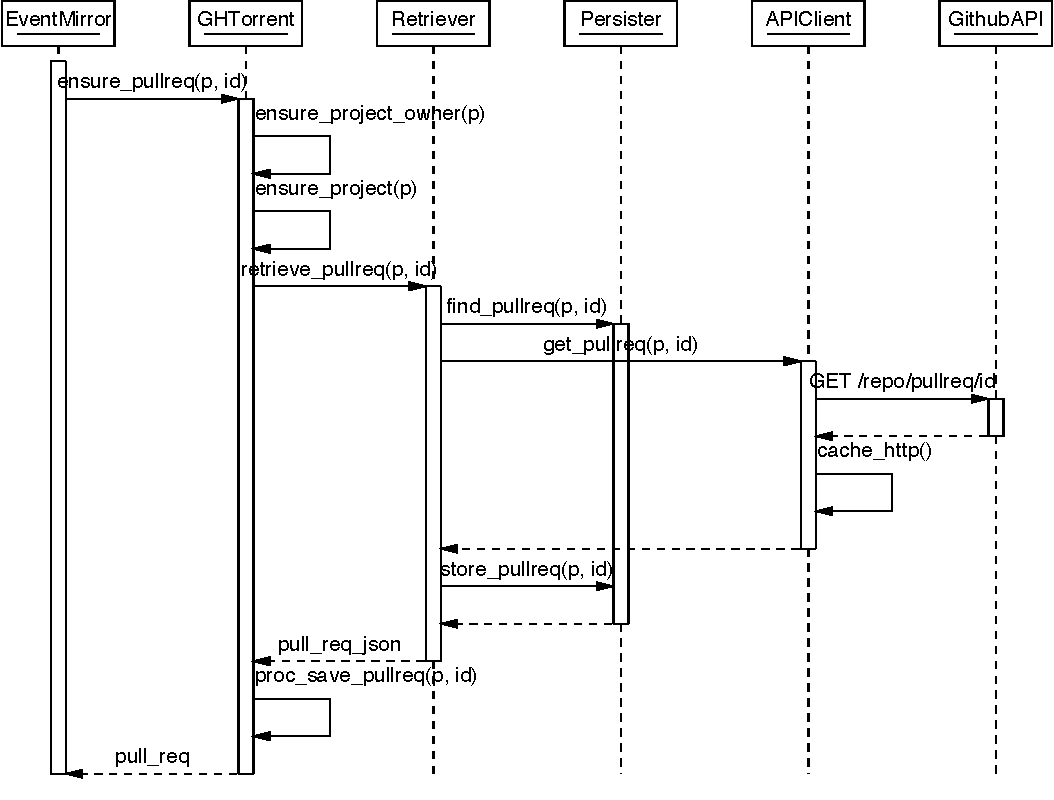
\includegraphics[scale=0.5]{ghtorrent-process.pdf} \end{center} \caption{The
%mirroring algorithm} \label{fig:mirror} \end{figure}
%
The mirroring algorithm is based on a recursive dependency resolution process.
For each retrievable item, we specify a set of dependencies, as they logically
flow from the data schema (see Figure~\ref{fig:entities}). For example, in order
to retrieve a \textsf{project}, it is necessary to retrieve the owning
\textsf{user} first; similarly, in order to retrieve a pull request, the
\textsf{project} needs to be retrieved first. If any step of the dependency
resolution fails, the whole item is marked as non-retrieved.  The process was
designed from start to be \emph{idempotent}: every step of the dependency
resolution may fail but once it succeeds, it will always return the same result.
This design choice has been very important since it makes our data stores append
only and the results of each step memoizable and therefore cachable.

\subsection{Data schema}

The data schema can be seen in Figure~\ref{fig:entities}. Following Github's
{\sc api} organization, most entities belong to a {\sf project} and contain
entries corresponding to actions initiated by a {\sf user}. The schema also
records information about {\sf users}, organizations and their members ({\sf
organization\_members}), while {\sf commits} are shared among {\sf projects}, their
forks, and {\sf pull\_requests}.  Most entities are timestamped with their
creation date (the \texttt{created\_at} field), while for entities which can be
in more than one states in time (e.g.,  {\sf pull\_requests} and {\sf issues}),
additional tables record those states in chronological order.  
For entities that correspond to {\sc api} calls, the \texttt{ext\_ref\_id}
field contains the unique identifier to the raw entity in the Mongo{\sc
db} database.

\subsection{Workers for Data}

The data collection was designed from the beginning as a decentralized process.
Decentralization is mediated using the worker queue model; a message producer
sends messages to the appropriate queue and several workers process messages,
perform the requests and store the results in the shared database.

Decentralization enables collaborating researchers to contribute to the data
collection effort, through what we call the \emph{workers for data} model.  In
exchange for data collection \emph{workers}, the project offers direct access to
the live project \emph{databases}. Set up instructions for workers as well as a
preconfigured virtual machine are offered through the project's web site. Apart
from offering direct access to the data, the project also distributes dumps of
the collected data, in both raw and relational formats. Depending on the use
case, the relational dump might be enough for further processing. The dumps are
distributed using the BitTorrent protocol. Furthermore, a query interface
allows third party users to directly query an archived version of the relational
database.

\section{Challenges and Limitations}

From a repository mining perspective, the {\sc ght}orent dataset has the following
limitations: 

\paragraph*{Data is additive} Github is a dynamic site where developers, 
    projects and wikis are created and deleted constantly. Despite the fact
    that the Github event stream reports additions of entities, it does
    not report deletions. This means that the information in the {\sc ght}orent 
    database cannot be updated when a user or a repository has been marked
    as deleted.

\paragraph*{Important entities are not timestamped}
\label{chal:timestamp}
Github does not report
    timestamps for the watchers/stars and followers entities. This means that it
    is not possible to query the followers for a user or the watchers for a
    repository at a specific timestamp. As a workaround, {\sc ght}orent uses the
    timestamp of the event that is generated when a follow/watch action is
    performed, but this is only limited to the events that took place since
    the {\sc ght}orent project started collecting data.


\paragraph*{Issues and pull requests} Issues and pull requests are dual on
Github; for each opened pull request, an issue is opened automatically.  Commits
can also be attached to issues to convert them to pull requests (albeit with
external tools). As a result, discussion comments for a pull request need to be
retrieved from multiple sources, namely from {\sf pull\_request\_comments} for
code reviews and from {\sf issue\_comments} for pull requests. Moreover, there
are two different status entities (namely, the pull request status and the issue
status) that need to be queried to get the succession of events on a pull
request.

\paragraph*{Commit users} Git allows users to setup custom user names as
    their commit names. The prevailing convention is that users use their email
    as their commit names; this is not a strict requirement though. By matching
    the commit email to the email the user has registered with at Github, it is
    possible for Github to report the same username across all entities
    (commits, issues, wiki entries, pull requests, comments etc) affected by a
    user. {\sc ght}orent relies on the git user name resolution to link an entry in
    the \textsf{users} table to an entry in the \textsf{commits} table. If the
    commit user has not been resolved, for example because a commit user is not
    a Github user or the git user's name is misconfigured, {\sc ght}orent will create
    a fake user entry with as much information as available. If in a future
    update, the resolution does take place, {\sc ght}orent will attempt to replace
    the fake entry with the normal entry. Despite this, there are several
    thousand fake users in the current dataset.
    
\paragraph*{Pull requests merged outside Github} Although Github
    automates the generation and submission of patches among repositories
    through pull requests, those need not be merged through the Github
    interface. Indeed, several projects choose to track the discussion on pull
    requests using Github's facilities while doing the actual merge using
    {\sf git}. This behaviour can be observed in projects where an usually big
    number of pull requests are closed without being reported as merged.
    In such cases, we can deduce that a pull request has been merged by checking
    whether the commits (identified by their {\sc sha} \texttt{id}) appear in 
    the main project's repository (through a metadata query). However, this
    heuristic is not complete, as several projects use commit-squashing or
    even diff-based patching to transfer commits between branches, thereby
    loosing authorship information.

%\subsection{Trivial projects} The majority of projects in Github are forks of
%    another project (54\% of the dataset). Of the remaining projects, several are
%    trivial, containing only a few commits, while many do not contain source
%    code (for example, Github pages repositories). To obtain a list of projects
%    worth investigating, the researcher should filter the remaining projects
%    for specific properties (for example, popularity, programming language etc).

\paragraph*{Issue tracking is open ended} Repository mining for bug tracking
    repositories is greatly enhanced, if records are consistent across
    projects. This is why most studies have been carried on Bugzilla data, which
    offers a good default set of properties per bug and little opportunities to
    customize the bug report further. On the other hand, Github's bug tracker
    only requires a textual description to open a bug. Bug property annotations
    (e.g. affected versions, severity levels) are delegated to project specific
    labels. This means that characteristics of bugs cannot be
    examined uniformly across projects.

\paragraph*{Changing data formats} As Github is in active development, the
provided data formats and {\sc api} endpoints are moving targets. During the
lifetime of the project, the commit entry schema changed twice, while the
\textsf{watchers} entity has been renamed to \textsf{stargazers}. We try to
follow the developments that affect the generation of our relational schema
only; so far, no modification was necessary.

\paragraph*{Some events may be missing} Malfunctions in the mirroring system
    (software or network) can result in some parts of the data that are missing.
    In principle, apart from events, all missing data in {\sc ght}orent can be
    restored (by replaying the event log or using the \texttt{ght-retrieve-repo}
    script) provided that the original data have not been deleted from Github.
    In the case of missing events, the current Github {\sc api} does not permit
    retrieving more than the 300 newest events per repository. On busy projects, this
    is less than a day's worth of event log. Known periods of missing events are
    several days at the beginning of March 2012, when an error to the event
    mirroring script went unnoticed, and from mid October 2012 to mid November
    2012, when we were trying to adapt {\sc ght}orent to the newly imposed
    requirement for authenticated {\sc api} requests.

\paragraph*{REST queries return modified results} Some {\sc rest api} calls
return slightly modified results if they are queried in different time 
moments. We have noticed this behaviour in the \texttt{created\_at} 
timestamps in several entities. In cases where the field is used as part
of a primary key, this might lead to duplicated records. Currently, this 
behaviour affects the \textsf{pull\_request\_history} and
\textsf{issue\_events}.

\section{Research Opportunities}

The {\sc ght}orent dataset is a rich source for both software engineering and
big data research; we outline some research opportunities emerging from
this data set below:

\subsubsection{Unified developer identities} {\sc msr} researchers have long
faced the
problem of disjoint developer identities when attempting to do research across
projects and data sources. The {\sc ght}orent dataset offers
combined source code, source code management, code review, issue and social
data using a single developer identity. Researchers can thus track developer
actions across projects (e.g. developer migrations) and combine them in 
novel and interesting ways. 

\subsubsection{Software ecosystems} In Github, project ecosystems are created
through forking, sharing of developers and dependency based linking of
components. The {\sc ght}orent dataset has rich, timestamped information about 
projects and their forks, which can be easily augmented with library
dependency information by automatically browsing related projects.

\subsubsection{Network analysis} Several networks are being formed on
Github, for example project networks through forks, developer networks
through participation to common projects, social networks through following
other users and watching repositories. Network analysis can either
be targeted, for example exploring project community formation dynamics, or
abstract by investigating the structure and stability of formed networks to
create predictors of future behavior network behavior.

\subsubsection{Collaboration and promotion} Researchers often ask questions
regarding the collaboration tactics of developers and membership promotion
strategies in {\sc oss} project organizations.  The {\sc ght}orent dataset,
provides timestamped data (albeit since the beginning of the {\sc ght}orent
project only, see Challenge~\ref{chal:timestamp} above) to investigate
how small contributions (known as ``drive-by commits'') and project
forking leads to developer and project collaboration and promotion of an
external developer to a team member.

\subsubsection{Replications of existing studies} A common theme in current
software engineering research is the lack of replications or the
mediocre replicability of existing works. The {\sc ght}orent dataset offers
an opportunity to replicate existing work and scale research to many
projects, as the dataset is homogenized across several thousand projects,
which can be queried for specific characteristics (e.g. programming language,
team size, presence of external collaborators etc).

\subsubsection{An extensible dataset} While {\sc ght}orent is covering all 
 public Github entities, it does not include advanced ways of
linking them yet. For example, projects can be linked by means of dependencies
in their build systems, while commits may be linked with issues by
searching for issue numbers in commit messages. The design of the
data update process in {\sc ght}orent makes such extensions possible:
database changes are tracked in a systematic way through migrations, while  
command line clients that exploit the distribution infrastructure are
trivial to develop. Collaborating researchers can thus extend the dataset
with custom analyses and data linking facilities.


\section{Related Work}

Similar to {\sc ght}orent is the Github Archive project~\cite{Grigo13}.  Both
projects mirror Github's public event timeline. The timeline sources are
different; while {\sc ght}orent uses the official Github {\sc api} timeline, Github
Archive parses the data used to create the corresponding Github web page.  Due
to the differences in the two {\sc api} endpoints, Github Archive's event
dataset is richer.  However, {\sc ght}orent also retrieves the data linked from the
event timeline, which allows it to go back in history; in fact, while Github
Archive's data starts in February 2012, {\sc ght}orent's dataset can and has been
extended for certain projects to 2008.  In addition, the {\sc ght}orent toolset
allows for retrieving the full history for a single project and the full list of
actions for a single developer, which may make it more appealing to the {\sc
msr} community.

\section{Conclusions}

In this work, we presented the {\sc ght}orent dataset and suite of tools, analyzed
the mirroring process and outlined the limitations of the current data.  The
provided dataset has a strong potential for providing interesting insights in
areas including but not limited to community dynamics, global software
engineering and distributed collaboration. We are actively seeking contributions
that will enhance the collected dataset's utility to the research community. 
More information can be found at \url{http://www.ghtorrent.org}.

The source code for the project can be obtained at \url{https://github.com/gousiosg/github-mirror}.

\section*{Acknowledgements}
This work is funded by Marie Curie {\sc ief} 298930 --- {\sc sefunc}.

\bibliographystyle{ieeetr}
\bibliography{ghtorrent-data}

\end{document}
